\section{Frontend}\label{sec:impl_frontend}
Frontendová část tohoto projektu zajišťuje především komunikaci mezi uživatelem a serverem pomocí prostředí, díky kterému je tato komunikace snazší a obecně přívětivější. Serverová část očekává příchozí požadavky od této části na cesty, které byly už definovány (viz sekce \ref{sec:routes}).

V~rámci této implementace (a z~podstaty využitých technologií) probíhá komunikace s~API (viz sekce \ref{sec:impl_backend}), které se tato část snaží poskytovat validní data. Slovo \uv{snaží} je zmíněno proto, jelikož se na ni v~reálném světe nemůžeme úplně spoléhat - frontendovou část může uživatel s~dostatečnými znalostmi a zkušenostmi modifikovat, čímž může i změnit způsob komunikace se serverem. To ale neznamená, že na ní nemůže probíhat jakákoliv validace a kontrola dat - frontend pro správnou funkčnost celé aplikace musí serveru ve výchozím (uživatelem nezměněném) stavu backendu poskytovat validní data - backend je ale musí preventivně validovat taky.

Uživatelské prostředí musí být připraveno tak, aby bylo příjemné k~užívání a ergonomické. Zároveň by nemělo být nějak složité a přehlcené ovládacími prvky, což by mohlo uživatele od používání aplikace odradit. Dále by toto prostředí mělo uživatele \uv{vést} úkonem, který chce uživatel provést - tzn. pokud zadává neplatná data, tak ho upozornit a rozhodně počkat na opravu dat před odesláním požadavku na server. Uživatelské prostředí, které v~rámci tohoto projektu vzniklo, je určeno primárně pro vykreslování ve webovém prohlížeči.

V~následující části jsou popsány jednotlivé frontendové komponenty a principy, díky kterým může celá aplikace fungovat.
	
	\subsection{Obecná struktura VueJS aplikace}\label{sec:obecna_str_vuejs}
	Nejprve je nutné rozebrat obecnou strukturu VueJS projektu.
	
	\begin{figure}[H]
		\centering
		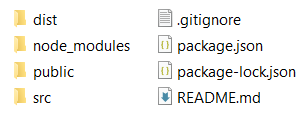
\includegraphics[width=0.6\textwidth]{img/vuejs_struktura.png} 
		\caption{Obecná struktura nově vygenerovaného VueJS projektu}
		\label{fig:vuejs_str}
	\end{figure}

	Jak můžeme na obrázku \ref{fig:vuejs_str} vidět, celý projekt je složen z~mnoha složek a souborů. Podrobný rozbor všech souborů a složek není předmětem této práce, proto jsou nejdůležitější zmíněné části popsány níže jen obecně.
	
	\begin{itemize}
		\item Složka \textit{dist} obsahuje zkompilovaný kód aplikace. \cite{FEDistFolder}
		\item Složka \textit{node\_modules} obsahuje závislosti a soubory přídavných balíčků NPM (viz sekce \ref{sec:npm}), které aplikace používá. \cite{VueJSFolder}
		\item Složka \textit{public} obsahuje obecně veřejné soubory (např. favicon). \cite{VueJSFolder}
		\item Složka \textit{src} obsahuje všechny soubory se zdrojovým kódem, ze kterých se poté tvoří zkompilovaný kód celé aplikace. \cite{VueJSFolder}
		\item Soubor \textit{package.json} obsahuje informace o~přídavných balíčcích spravovaných pomocí NPM (viz sekce \ref{sec:npm}). \cite{VueJSFolder}
	\end{itemize}
	
	Popsaná struktura výše je standardní pro oddělenou frontendovou aplikaci. To v~implementaci tohoto projektu ale neplatí, jelikož je frontend přímo zaintegrován v~Laravel projektu (viz sekce \ref{sec:strukura_laravel}). Jsou zde tyto rozdíly:
	
	\begin{itemize}
		\item Složka \textit{src} je nahrazena složkou \textit{js} ve složce \textit{resources}.
		\item Složka \textit{public} je umístěna v~kořenovém adresáři Laravel projektu a je sloučena se složkou \textit{dist}.
		\item Složka \textit{node\_modules} společně se souborem \textit{package.json} je také umístěna v~kořenovém adresáři Laravel projektu.
	\end{itemize}
	
	Celkovou administrativu nad celým VueJS projektem poté zajišťuje modul Laravel Mix podle konfiguračního souboru webpack.mix.js \cite{LaravelMixVue}. Ten je také umístěn v~kořenovém adresáři projektu. Díky celému tomuto přístupu může backend i frontend běžet jako jedna aplikace na jedné doméně.
	
	Jak již bylo zmíněno, zdrojový kód, tedy nejdůležitější část frontendové aplikace, leží standardně ve složce \textit{src} - v~tomto projektu ve zmíněné složce \textit{js}. Oproti běžné samostatné VueJS aplikaci je zde (ve složce \textit{js}) největší rozdíl v~pojmenování souborů - soubor \textit{main.js} byl přejmenován pro potřeby Laravelu na \textit{app.js}. Také se navíc v~této složce nachází Laravelem vygenerovaný soubor bootstrap.js pro další konfiguraci při kompilaci. Nakonec byla kvůli nevyužití odebrána složka \textit{assets} a pro další účely přidána složka \textit{apis} (viz obrázek \ref{fig:zdroj_kod_vue_rozdily}).
	
	\begin{figure}[h]
		\centering
		\subfloat[\centering]{{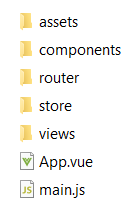
\includegraphics[height=5cm]{img/zdroj_kod_vue/src.png} }}
		\qquad
		\subfloat[\centering]{{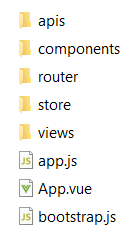
\includegraphics[height=5cm]{img/zdroj_kod_vue/js.png} }}
		\caption{Porovnání obsahu složek \textit{src} (a) a \textit{js} (b)}
		\label{fig:zdroj_kod_vue_rozdily}
	\end{figure}

	Každý soubor a složka ve zmíněném adresáři \textit{js} má určitý význam. Ty jsou představeny níže (soubor bootstrap.js byl již popsán výše). Další rozbor jednotlivých souborů ve zmíněných složkách je obsažen v~dalších sekcích této práce.
	\begin{itemize}
		\item Složka \textit{apis} obsahuje prostředky pro komunikaci s~API (tedy s~backendem).
		\item Složka \textit{components} obsahuje všechny komponenty, které jsou využívány v~celé aplikaci.
		\item Složka \textit{router} obsahuje prostředky pro přesměrovávání a definování cest ve frontendové aplikaci.
		\item Složka \textit{store} obsahuje nástroje pro držení dat ve webovém prohlížeči.
		\item Složka \textit{views} obsahuje veškeré pohledy, na které se můžeme pomocí definované cesty dostat.
		\item Soubor \textit{app.js} je kořenový soubor aplikace shromažďující všechny reference na ostatní soubory (zabaluje celou aplikaci).
		\item Soubor \textit{App.vue} je kořenová šablona, která přijímá pohledy na základě cesty, které poté vykresluje (tvoří aplikační kostru HTML).
	\end{itemize}

		\subsubsection{Souhrn využitých balíčků}\label{sec:fe_packages}
		Pro přehlednost je zde vytvořena kapitola shrnující vybrané externí balíčky, které byly do frontendové části přidány, a jejich základní účel a funkcionalita.
		
		\begin{itemize}
			\item Balíček \uv{@braid/vue-formulate} (dále jako VueFormulate) je použit pro veškeré formulářové prvky. Kromě zprostředkování hotových komponent pro jednotlivé elementy formuláře také nabízí např. validaci dat.
			\item Balíček \uv{vue-chartjs} (zastřešující populární balíček \uv{chart.js}) je použit pro grafické vyobrazení dat ve formě grafů.
			\item Balíček \uv{randomcolor} je použit pro generování náhodných barev (využito u~grafů k~dynamickému rozlišení dat).
			\item Balíček \uv{uuid} je použit pro generování unikátního identifikátoru (především funkce \textit{uuidv4}, např. u~vytváření formuláře k~označování vytvořených otázek).
			\item Balíček \uv{vue-js-modal} je použit k~vytváření a správě modálních oken.
			\item Balíček \uv{vue-toasted} je použit pro zobrazování zpráv o~průběhu různých činností (např. zobrazení chybových hlášek).
		\end{itemize}
	
		Dále frontend obsahuje reference na automaticky přidané balíčky, které nejsou předmětem této práce. Lze z~nich ale vyjmout např. \uv{vuex} a \uv{vuex-persist} (správa držení dat v~prohlížeči), \uv{vue-router} (správa cest mezi jednotlivými částmi aplikace - směrovač) či \uv{axios} (komunikace s~API).
	
	\subsection{Komunikace s~Laravel API}\label{sec:komunikace_s_api}
	Komunikace mezi frontendovou aplikací a Laravel API je pro celkovou funkčnost projektu klíčová - bez ní by nedávala existence této části žádný smysl. K~těmto účelům je do projektu přidán balíček \uv{axios} - ten se stará o~veškerou komunikaci mezi klientskou a serverovou stranou tzn. data dokáže odesílat i přijímat. Komunikace probíhá tak, že nějaký frontendový prvek (obvykle pohled) volá metody zastřešené tímto balíčkem a na základě odpovědi ze serveru dostává data.
	
	Všechny tyto metody a soubory spojené s~komunikací se nachází ve složce \textit{apis}. Zde je klíčový soubor \textit{Api.js}, ve kterém nejprve inicializujeme objekt, který celou komunikaci zastřešuje (ten pochází ze zmíněného balíčku) - tomu je vhodné přiřadit výchozí cestu, ze které bude později tvořit absolutní cesty, na které bude posílat specifické požadavky (v~případě této implementace název domény + řetězec \textit{/api/}). Poté mu deklarujeme, co má provést v~případě příchozí odpovědi ze serveru bez chyby a s~chybou. V~případě úspěšné akce (tedy navrácení dat bez chyby - obvykle s~kódem 200) jsou data bez jakýchkoli úprav předána komponentě, která si je žádala. V~opačném případě (tedy při chybě) je kromě vrácení obsahu příchozí zprávy také do konzole vypsána příslušná chyba. Vrácení příchozích dat s~chybou tímto způsobem je určeno pro vytvoření chybového oznámení pro uživatele - aby uživatel věděl, proč daná operace selhala. Zároveň to slouží např. samotným pohledům - na základě chybové hlášky nebo chybového stavového kódu přizpůsobí své chování. Výpis do konzole sloužil primárně k~vývoji aplikace - ničemu ale nevadil, proto byl v~aplikaci ponechán. 
	
	Speciálním případem je situace, kdy se vyskytne chyba se stavovým kódem 401 nebo 419 (uživatel pravděpodobně chce přistoupit k~obsahu, ke kterému nemá v~současnou chvíli oprávnění např. protože mu vypršela relace přihlášení). V~takovém případě se aplikace pokusí uživateli zneplatnit přihlášení a odstranit o~něm záznam z~prohlížeče a uživatele automaticky přesměrovat na pohled pro přihlášení.
	
	Další soubory ve zmíněném adresáři jsou \textit{Form.js} a \textit{User.js}. Ty obsahují konkrétní funkce s~referencí na objekt deklarovaný v~souboru \textit{Api.js}, přednastavenou metodu komunikace (ta musí korelovat s~metodami na API viz sekce \ref{sec:routes}) a relativní cestu, na kterou budou požadavek směrovat (ta je spojena s~předem definovanou výchozí cestou). Zmíněné cesty samozřejmě musí odkazovat na existující cesty definované serverem (viz tabulky \ref{tab:verejne_cesty} a \ref{tab:cesty_s_prihlasenim}). Funkci je samozřejmě možné předat parametr (obvykle set dat), který je poté předán na server. Jak už z~názvů souborů vyplývá - \textit{Form.js} zaštiťuje komunikaci týkající se manipulace s~formuláři nebo s~odpověďmi na formulář a \textit{User.js} zajišťuje komunikaci v~rámci veškeré administrativy nad uživateli.
	
	\subsection{Komponenty}\label{sec:komponenty}
	Komponenty jsou v~podstatě \uv{díly k~složení celé aplikace}. Díky nim nemusíme např. stránku pro vytvoření formuláře psát do jednoho nepřehledného a obrovského souboru, ale můžeme tento kód rozdělit. Výhodou také je, že když budeme tento komponentový styl zápisu kódu dodržovat, lze jeho části v~jiných místech opětovně využít - předcházíme tím redundantnímu kódu, který zbytečně znepřehledňuje celý projekt. Všechny zmíněné komponenty jsou zapsány v~souborech s~koncovkou \textit{.vue} a disponují stejným jménem jako samotný soubor. Struktura kódu je vyobrazena v~obrázku \ref{fig:vue_kod_komponenty}.
		
		\subsubsection{Základní komponenty} \label{sec:komp_zakl} %Header, Loading, teor. App.vue
		Mezi základní komponenty jsou řazeny především ty, jejichž použití se opakuje v~aplikaci nejčastěji - tedy \textit{Header} a \textit{Loading}. 
		
		Komponenta \textit{Header} slouží k~vykreslení horního navigačního panelu s~nabídkou dalších funkcionalit, který na základě přihlášení uživatele mění svůj obsah. Pokud není nikdo přihlášen, nabídka nabízí odkazy na přihlášení či registraci. Pokud se uživatel přihlásí, může se odsud dostat na stránku svého profilu, na vytvoření nového formuláře nebo se odhlásit ze svého účtu.
		
		Komponenta \textit{Loading} obsahuje jednoduchou animaci, která symbolizuje průběh načítání. Je využita v~částech komponent a pohledů, kde je očekáván např. příjem nějakých dat z~backendu, na který se musí čekat. Uživateli má vyobrazovat, že v~aplikaci probíhá nějaká činnost.
		
		Dále zde lze zmínit i komponentu \textit{App} z~kořenového adresáře frontendu, která již byla popsána v~sekci \ref{sec:obecna_str_vuejs}. Lze dodat, že se v~ní kromě předaných pohledů nachází i reference na komponentu \textit{Header} - ta musí být z~podstaty věci vykreslena na všech cestách.
		
		\subsubsection{Komponenty elementů formuláře} \label{sec:komp_form} %Elements, FormElement...*
		Tyto komponenty představují jednotlivé otázky a k~ním příslušný vstup definovaný typem (pokud se nejedná o~element nové stránky). Existují zde interaktivní komponenty elementů (použity např. ve vyobrazení celého formuláře k~vyplnění) nebo komponenty statické (použity např. ve vyobrazení jednotlivých otázek při vytváření formuláře).
		
		Interaktivní komponenty elementů formuláře nalezneme v~podsložce \textit{Elements} - zde se nachází tyto komponenty: \textit{BooleanInput}, \textit{DateInput}, \textit{NumberInput}, \textit{SelectInput} a \textit{TextInput} (vycházející z~typů ze sekce \ref{sec:form_inputs_types}). Všechny tyto komponenty jsou si navzájem velmi podobné. Všechny využívají komponenty z~balíčku \uv{VueFormulate}: \textit{FormulateInput} pro vykreslení samotné otázky a vytvoření vstupního pole podle datového typu pro odpověď (např. pro text je vygenerována oblast, do které lze vkládat textový řetězec) a \textit{FormulateErrors} pro výpis validační chyby (např. pokud má mít vkládaný text délku maximálně deset znaku a do oblasti vstupu je vložen text delší, tak se objeví chybové hlášení pod otázkou). V~logické části jsou si taktéž všechny komponenty podobné - při jejich inicializaci se na základě přijmutích dat nastaví validační pravidla pro vstup a ID otázky, ke které samotná komponenta patří.
		
		Tyto interaktivní komponenty jsou poté zabaleny do dalších komponent. Komponenta \textit{FormElement} na základě příchozích dat (tj. typ otázky) vrací rodičovské komponentě \textit{FormElementsComponent} příslušný element formuláře rozebraný v~předchozím odstavci. Zmíněná rodičovská komponenta poté figuruje především při vykreslování celého formuláře - má za úkol vykreslovat veškeré otázky formuláře s~funkcí stránkování. Při inicializaci této komponenty se otázky nejprve rozdělí do příslušných polí, které představují stránky, na základě výskytu elementu nové stránky (tzn. pokud se při procházení všech elementů formuláře najde element nové stránky, tak je vytvořeno nové pole, do kterého se přesouvají další otázky). Po vzniku těchto polí představující stránky dojde k~jejich vykreslení pomocí zmíněné komponenty \textit{FormElement}. Stránkování je zde zajištěno pomocí skrývání a odkrývání jednotlivých stránek pomocí CSS stylů ovládaných příslušnými tlačítky - takto to je řešeno kvůli udržení dat při přesunu na další stránku (nutné opatření kvůli zmíněnému balíčku k~tvoření formulářových prvků).
		
		V~rámci statických komponent zde existuje komponenta \textit{FormElementControl}. Ta slouží k~vykreslování reprezentace otázek nebo elementu nové stránky v~pohledech vytváření nebo úpravě formuláře. Jedná se o~komponentu, která na základě předaného typu elementu (tj. otázka s~příslušným typem nebo nová stránka) vrací příslušnou reprezentaci elementu (např. v~případě textového vstupu vyobrazení textového pole, do kterého nelze vyplňovat, a samotné otázky). Při kliknutí na element otázky se objeví modální okno pro úpravu vybrané otázky - toto modální okno je popsáno dále v~práci. U~elementu nové stránky toto provést nelze, proto je zde připraven jen prokliknutelný text \uv{Remove}, který vysílá specifickou událost do rodičovské komponenty, která ho používá (slouží k~odebrání elementu).
	
		\subsubsection{Modální okna} \label{sec:komp_modal} %Modals
		Zmíněné komponenty představují předpis vykreslení pro modální okna spravovaná balíčkem \uv{vue-js-modal}. Na jejich funkčnosti závisí několik pohledů. Tyto komponenty se nachází v~podsložce \textit{Modals} - zde existují ještě další tři podsložky pojmenované podle oblasti, ve které jsou používány. Ty poté obsahují příslušné soubory komponent. Jedná se tedy o~tyto složky: \textit{CreateForm}, \textit{FormResults}, \textit{FormReview}. 
		
			\subsubsubsection{Manipulace s~elementy formuláře}
			První adresář \textit{CreateForm} obsahuje příslušné komponenty modálních oken a podkomponenty využívané především v~pohledu vytváření formuláře. Později byly tyto komponenty využity i v~pohledu pro úpravu formuláře - název tohoto adresáře se ale neměnil. Adresář obsahuje komponenty modálních oken \textit{ItemModal} a \textit{SelectChoiceModal}.
			
			Komponenta \textit{ItemModal} slouží k~samotné tvorbě nového elementu nebo úpravě stávajícího elementu otázky ve formuláři - to je možné pomocí manipulace s~dočasným úložištěm dat \textit{createFormStore} (viz \ref{sec:data_prohlizec_form}), se kterým se pracuje např. v~rodičovském pohledu pro vytváření formuláře. K~manipulaci s~daty využívá příslušné metody inicializovaného úložiště.
			
			Celé modální okno je zobrazeno na základě vyžádání rodičovského prvku (např. pohledu pro vytvoření formuláře) a je tvořeno zejména komponentou \textit{FormulateForm} (z~balíčku \uv{VueFormulate}), ve které jsou vnořeny všechny ovládací prvky (tvořené komponentami \textit{FormulateInput} a \textit{FormulateErrors}) - ty shromažďují veškeré informace o~elementu otázky - tedy typ odpovědi na otázku (např. text nebo číslo), samotnou otázku, zda je otázka povinná a další validační pravidla, která jsou vázána na typ otázky (tato pravidla vychází ze sekce \ref{sec:form_inputs_types}). Ovládací prvky dalších validačních pravidel jsou další samotné komponenty připojované do modálního okna - každý typ otázky má pro tyto účely svou podkomponentu (jedná se o~\textit{DateItem}, \textit{NumberItem}, \textit{SelectItem} a \textit{TextItem} ve stejné složce). Tyto prvku mohou být už předvyplněny v~situaci, kdy je upravován existující element (komponenta může přijímat vstupní hodnoty). Data jsou poté na základě stisknutí příslušného tlačítka (např. s~účelem vytvoření nového elementu s~textem \uv{Create}) z~modálního okna předána příslušné metodě úložiště, která si data sama zpracuje.
			
			Známou komplikací je samozřejmě zpracování otázek s~možnostmi odpovědi. K~těmto účelům je v~komponentě \textit{SelectItem} vnořena další podkomponenta \textit{SelectChoicesComponent}. Tato komponenta poskytuje administrativu nad možnostmi odpovědi - k~tomu používá vlastní dočasné úložiště \textit{createFormChoicesStore}, které má stejné metody jako již zmíněné úložiště \textit{createFormStore} (data z~celé této komponenty samozřejmě podléhají i manipulaci s~daty rodičovské komponentě \textit{ItemModal}). V~komponentě jsou kromě tlačítka pro přidání možnosti odpovědi vykreslovány možnosti odpovědi. Ty lze samozřejmě modifikovat - při kliknutí na ně se zobrazí další modální okno \textit{SelectChoiceModal}, ve kterém ji lze upravit příslušné hodnoty (toto okno je používáno i k~přidávání těchto možností). Toto okno poté data předává zmíněnému poskytnutému úložišti. Zajímavou funkcí, kterou lze u~\textit{SelectChoicesComponent} zmínit, je hlídání hodnoty \textit{hasHiddenLabel} pocházející z~rodičovské komponenty (ta značí, zda možnosti odpovědi mají skrytý popisek - tj. škála) - pokud je tato hodnota změněna z~\textit{true} na \textit{false}, tak jsou automaticky tyto skryté popisky odstraněny. V~opačném případě komponenta automaticky očísluje možnosti odpovědi čísly 1,2,3,...
			
			\subsubsubsection{Výsledky formuláře}\label{sec:modalni_okna_vysledky_form}
			Dalším adresářem je \textit{FormResults} obsahující pouze jedno modální okno s~názvem \textit{FormResultsPublicationModal}. To je využito zejména v~pohledu pro zobrazení výsledků formuláře. Toto okno je znovu tvořeno především prvky z~balíčku \uv{VueFormulate}. 
			
			Před inicializací přijímá všechny otázky formuláře, hodnotu vyjadřující zda je formulář už zveřejněn a identifikátor formuláře. Poté, na základě přijatých dat, vypisuje jeho současný stav a možnosti, co lze s~formulářem provést. Klíčová je hodnota vyjadřující zda jsou už výsledky veřejné - pokud se rovná \textit{false}, je zobrazeno jen prázdné zaškrtávací políčko vyjadřující, že výsledky zveřejněny nejsou. Pokud se hodnota rovná \textit{true}, jsou vypsány i všechny otázky, u~kterých lze označit, která z~nich bude veřejně viditelná. Zmíněnou hodnotu můžeme pomocí zaškrtávacího políčka samozřejmě měnit - s~tím se i dynamicky změní rozložení okna. Poté, co navolíme příslušné parametry a klikneme na tlačítko pro uložení nastavení, je na server poslán požadavek s~příslušnými údaji. Ten je zpracován metodou \textit{publishResults}, která je popsána v~sekci \ref{sec:form_publish_results}. Po úspěšném provedení činnosti se okno zavírá a celá stránka je přenačtena.
			
			\subsubsubsection{Manipulace s~celým formulářem}\label{sec:modalni_okna_man_form}
			Posledním adresářem je \textit{FormReview}. Ten obsahuje dvě modální okna použitá v~pohledu pro zobrazení souhrnu informací o~formuláři. Jedná se o~komponenty \textit{FormAccessibilityModal} a \textit{FormDuplicationModal}.
			
			Komponenta \textit{FormAccessibilityModal} slouží k~úpravě přístupnosti formuláře. Je také tvořena především komponentami z~balíčku \uv{VueFormulate} a ke svému správnému chodu potřebuje při vytvoření nejprve dostat hodnotu vyjadřující současnou přístupnost (zda je formulář veřejný nebo privátní) a identifikátor formuláře - pokud se jedná o~privátní formulář, musí být předány i emaily, na které byla už zaslána pozvánka. Na základě těchto dat je vykresleno příslušné rozložení modálního okna - toto rozložení lze měnit na základě změny hodnoty vyjadřující přístupnost. Pokud je zmíněná hodnota \textit{false}, zobrazí se jen související prázdné zaškrtávací políčko. Pokud se ale rovná \textit{true}, zobrazují se zde i další dva ovládací prvky. V~prvním lze vidět emaily, na které již byla zaslána pozvánka - ty lze pro zneplatnění pozvánky označit. V~druhém můžeme zase přidat emaily, na které bude poslána nová pozvánka k~vyplnění formuláře. Nakonec (po kliknutí na tlačítko vyjadřující provedení změny) se příslušná data pošlou na server. Ta jsou zpracována metodou \textit{updateAccess}, která je popsána v~sekci \ref{sec:form_accessibility}. Modální okno se poté zavře a stránka je přenačtena.
			
			Druhá komponenta \textit{FormDuplicationModal} nám umožňuje duplikovat vybraný formulář. I~toto modální okno je tvořeno komponentami z~balíčku \uv{VueFormulate} a při inicializaci očekává základní data o~formuláři - tedy jeho název, popisek, datum zveřejnění, datum ukončení zveřejnění a zda se jedná o~formulář veřejný či privátní (u~privátního také emaily, které dostali pozvánku). Tato data jsou dočasně uložena v~úložišti \textit{duplicateFormStore}, které je popsáno v~sekci \ref{sec:data_prohlizec_form}. Tyto údaje lze libovolně měnit - pokud jsou zadány neplatné hodnoty (např. datum zveřejnění je dále v~čase než datum ukončení zveřejnění), tak nás okno bude informovat příslušným upozorněním. Poté, co klikneme na příslušné tlačítko pro duplikaci formuláře, je odeslán na server požadavek, který je vyřízen metodou \textit{duplicateWithAuth}, jež je popsána v~sekci \ref{sec:form_dupl}. Po tomto úkonu je modální okno zavřeno a stránka přenačtena.
		
		\subsubsection{Komponenty pro zobrazení výsledků} \label{sec:komp_vysledky} %ResultComponents
		Dalšími komponentami, které jsou zde popsány, jsou komponenty pro grafické znázornění dat v~pohledu pro zobrazení výsledků formuláře (pro vyobrazení dat ve formě grafů zde byl použit balíček \uv{vue-chartjs}). Nachází se v~adresáři \textit{ResultComponents}, který obsahuje komponenty \textit{DetailedResultsTable}, \textit{ResultComponent} a \textit{ResultRender}. Také se zde nachází podsložka \textit{Views}, ve které lze najít předpřipravené podkomponenty pro konkrétní styl vykreslení dat - \textit{Bar} pro vykreslování sloupcových grafů, \textit{List} pro vykreslování jednoduché tabulky stylem klíč/hodnota (resp. ID odpovědi/odpověď) a \textit{Pie} pro vykreslování koláčových grafů. Tyto podkomponenty jsou poté předávány dál pomocí zmíněné komponenty \textit{ResultRender}, která je vrací na základě předaného typu a dat (tzn. výsledky z~otázek s~možnostmi odpovědi nebo z~otázek Ano/Ne jsou zobrazovány jako grafy - lze si mezi zmíněnými styly grafu po načtení vybrat, ostatní jako zmíněná tabulka).
		
		Popsaná komponenta \textit{ResultRender} je poté využita ve zmíněné komponentě \textit{ResultComponents}. Pro správnou funkcionalitu komponenta \textit{ResultComponents} musí pro získání příslušného vyobrazení dat samozřejmě předaná data zpracovat do validního formátu a poté je poskytnout komponentě \textit{ResultRender}. Nakonec zmíněná rodičovská komponenta \textit{ResultComponents} přidá k~vyobrazení dat (např. ve formě grafu) samotnou otázku a celý obsah je předán do pohledu pro zobrazení výsledků.
		
		Nelze opomenout komponentu \textit{DetailedResultsTable}, která slouží jako alternativní zobrazení všech výsledků formuláře. (ve výchozím nastavení se zobrazují data ve zmíněných grafech nebo v~tabulce pro každou otázku). V~podstatě data zobrazuje v~podobném formátu, jako jsou vysázeny při exportu dat (tzn. v~tabulce viz sekce \ref{sec:form_comp_export}). Oproti exportu se vyobrazení dat liší v~tom, že v~buňkách, kde není žádná hodnota (\textit{null}), tam je umístěn znak pomlčky (\uv{-}).
		
		\subsubsection{Komponenta karty formuláře}\label{sec:fe_komp_karta_form}
		Jednoduchá komponenta, kterou nebylo možné zařadit mezi ostatní výše, s~názvem \textit{FormCard} slouží jako předpis pro vykreslování karty formuláře. Ta je použita v~pohledu úvodní stránky v~případě, že je uživatel přihlášen a že už nějaké formuláře vlastní. Po kliknutí na kartu se přihlášený uživatel dostane na pohled se zobrazením souhrnu informací o~požadovaném formuláři. Sama o~sobě karta zobrazuje název a popisek formuláře či data spuštění a ukončení zveřejnění formuláře.
	
	\subsection{Směrovač}\label{sec:fe_router} %%Router
	K~tomu, abychom mohli přecházet mezi částmi aplikace, je nutné, aby v~aplikaci existoval nějaký komplexní systém, který by nad tímto problémem měl kontrolu. To zde řeší tzv. směrovač (běžně známý pod anglickým názvem Router), který je importován z~balíčku \uv{vue-router}. Tento směrovač má za úkol na základě definovaných možných cest v~aplikaci vracet příslušný pohled uživateli.
	
	Směrovač implementovaný v~tomto projektu je umístěn ve složce \textit{router} v~souboru \textit{index.js}. V~tomto souboru jsou nejprve vydefinovány všechny relativní cesty, ke kterým je přiřazen hlavně příslušný pohled, který je při vstupu na nějakou z~cest vrácen uživateli - některé mohou disponovat i metadaty (např. zda cesta vyžaduje pro vykreslení přihlášení uživatele). Poté je inicializován objekt tohoto směrovače, kterému jsou předány především data jako výchozí cesta (v~této implementaci název domény), ke které jsou relativní cesty ve výsledku připojeny, a samotná kolekce vydefinovaných cest. 
	
	Nakonec lze určit i specifické chování pro zmíněná metadata u~cest, což je zde také využito a popsáno níže:
	\begin{itemize}
		\item Pokud cesta vyžaduje přístup bez přihlášení a uživatel je přihlášen, je přesměrován na domovskou stránku (např. pokus o~přístup na přihlašovací stránku). Pokud není přihlášen, je přesměrován na stránku na zvolené cestě.
		\item Pokud cesta vyžaduje přístup s~přihlášením a uživatel je přihlášen, je přesměrován na stránku na zvolené cestě. Pokud není, je přesměrován na pohled pro přihlášení (např. pokus o~přístup na pohled zobrazující souhrn informací o~formuláři, který je určen jen přihlášenému majiteli formuláře).
		\item Pokud nemá cesta žádná známá metadata, je uživatel přesměrován na stránku na zvolené cestě.
	\end{itemize}

	\subsection{Držení dat v~prohlížeči} %% Store
	Možnost držení dat v~prohlížeči je další ze základních atributů pro správnou funkčnost aplikace. Ať už se jedná o~soubory cookies nebo o~dočasné úložiště v~paměti alokované přímo JavaScriptem - jednoduše je to potřeba. V~tomto projektu byly využity oba zmíněné přístupy.
	
	Soubory spojené s~držením dat pomocí JavaScriptu (označovány jako Stores) jsou umístěné ve složce \textit{store} - jedná se o~soubor \textit{index.js} a soubor \textit{MyStoreClass.js}.
	
		\subsubsection{Přihlášení uživatele}
		V~rámci přihlášení uživatele lze držení dat rozdělit na dvě větve: pomocí cookies a pomocí držení dat v~JavaScriptu za využití balíčku \uv{vuex}. 
		
		V~cookies jsou drženy šifrované tokeny, které jsou spravované přímo backendovým balíčkem pro zabezpečení single-page aplikací \uv{Laravel Sanctum} a slouží k~ověřování přihlášení (jsou autonomně posílány společně s~každým požadavkem na server - ten na základě jejich platnosti provede požadovaný úkon). 
		
		Naproti tomu přihlášení drženo pomocí \uv{vuex} je zde primárně pro funkčnost metadat u~směrovače (viz sekce \ref{sec:fe_router}) - na základě tohoto drženého stavu může přihlášený uživatel přistupovat na stránky, které jsou přístupné pouze s~přihlášením. Toto je definováno v~souboru \textit{index.js}, kde probíhá inicializace objektu z~balíčku \uv{vuex}, který má deklarován příslušné proměnné držící stav (states), metody pro vrácení hodnot proměnných držících stav (getters), metody pro cílenou změnu hodnot (mutations) a další procedury ve formě metod (actions - např. procedura pro přihlášení uživatele). K~tomu, aby data nebyla smazána při přenačtení stránky, musí být přidán zmíněnému objektu plugin \textit{VuexPersistence} z~balíčku \uv{vuex-persist}, který toto chování zprostředkovává.
		
		\subsubsection{Data pro manipulaci s~formuláři}\label{sec:data_prohlizec_form}
		K~tomu, abychom mohli vytvářet, upravovat nebo duplikovat formuláře, bylo nutné jejich data dočasně (do odeslání požadavku na server) držet v~prohlížeči. K~těmto účelům vznikla tři dočasná \uv{skladiště} dat - \textit{createFormStore}, \textit{createFormChoicesStore} a \textit{duplicateFormStore}.
		
		První dva zmíněné objekty (tedy \textit{createFormStore} a \textit{createFormChoicesStore}) jsou určené pro vytváření a úpravu formuláře a jsou ve své podstatě naprosto identické, jelikož se jedná o~instance pro projekt vytvořené třídy \textit{MyStore}, která se nachází v~souboru \textit{MyStoreClass.js}. Třída \textit{MyStore} obsahuje proměnnou pro ukládání dat, což je objekt, ve kterém je vytvořeno pole pro ukládání hodnot kolekce dat. Kromě této proměnné třída disponuje různými metodami: \textit{getItems} vrací všechny prvky kolekce, \textit{addItem} ukládá předaná data z~parametru do kolekce, \textit{refreshItemsOrder} obnovuje hodnotu pořadí každému prvku v~kolekci (tzv. postupně očísluje prvky), \textit{sortItemsByOrder} řadí prvky v~kolekci podle hodnoty pořadí, \textit{changeItem} dokáže nahradit existující prvek v~kolekci na základě shody ID, \textit{deleteItem} smaže prvek z~kolekce na základě ID, \textit{clearStore} vymaže všechny prvky z~kolekce a \textit{setItems} přepíše celou kolekci předanou kolekcí.
		
		Třetí objekt (\textit{duplicateFormStore}) slouží k~držení dat pro duplikaci formuláře. Oproti zmíněným instancím se jedná o~\uv{skladiště}, které je připraveno pro konkrétní data související s~duplikací. V~rámci proměnných, ve kterých dočasně drží data, jsou zde vlastně deklarovány pole pro příslušné ovládací prvky modálního okna pro duplikaci (viz sekce \ref{sec:modalni_okna_man_form}). Dále obsahuje standardní metody pro smazání, přepsání a vrácení uložených dat (\textit{clearData}, \textit{setData} a \textit{getData}), ale také metodu pro validaci těchto dat (\textit{validateData}, která na vrací případnou chybovou hlášku pro zobrazení v~modálním okně) či metodu pro zjištění, zda je úložiště prázdné neboli ve výchozím stavu (\textit{isStoreEmpty}).
		
		Lze namítat, že pro ukládání těchto dočasných dat je možné využít lokální úložiště VueJS komponenty \textit{data} - zde to ale možné nebylo, jelikož bylo potřeba předávat data mezi více komponentami. Zároveň, díky tomuto přístupu, jsem mohl s~daty manipulovat v~určitých situacích jednodušeji za pomocí předpřipravených metod.
	
	\subsection{Pohledy}
	Pohledy (anglicky Views) jsou v~rámci struktury kódu stejné jako komponenty, které jsou popsány v~sekci \ref{sec:komponenty}. Nacházejí se ve složce \textit{views} a ve své podstatě i oni jsou komponentami - rozdíl je jen ve využití, jelikož pohledy jsou skládány ze zmíněných komponent. Poté, co je pohled složen z~těchto komponent, je vykreslen jako plnohodnotná stránka. U~samostatných komponent nemá význam, aby byly vykreslovány samostatně - potřebují data ke zpracování, která jim předává právě pohled. 
	
	Jak již bylo řečeno, pohled musí podřadným komponentám, které implementuje, dodat data ke správné funkčnosti. Tato data získává pomocí komunikace s~API na základě volané metody a předaných dat (viz sekce \ref{sec:komunikace_s_api}). Poté, co získá odpověď ze serveru, tak před předáním komponentám data obvykle zpracuje do takového formátu, který komponenty očekávají. Zároveň řeší i situace, kdy dojde k~chybě při přijmu dat - pohled musí dát samozřejmě uživateli vědět příslušným způsobem, co se v~aplikaci stalo resp. proč např. nedostal data, která požadoval. Zároveň pohled obsahuje příslušné ovládací prvky, které nám umožňuji se pohybovat mezi pohledy - toto je zajištěno směrovačem, který je popsán v~sekci \ref{sec:fe_router}.
	
	V~této části jsou obecně popsány všechny komponenty a jejich účel. V~částech, kde jsou použity vstupní ovládací prvky (např. pro zadání textové hodnoty), jsou data před posláním na sever také náležitě validována (např. validací, kterou poskytují komponenty z~balíčku \uv{VueFormulate}). Pohledy jsou responzivní - obrázky v~této práci byly snímány v~rozložení pro tablet. 
		
		\subsubsection{Domovská stránka} %% Home
		První pohled, který je zobrazen uživateli především při prvním použití aplikace nebo ihned po přihlášení, je právě pohled domovské stránky (viz obrázek \ref{fig:pohled_home}). Tento pohled je rozdělen na dva způsoby vykreslení - bez přihlášení a s~přihlášením.
		
		Pokud uživatel přihlášený není, je zobrazena úvodní stránka, která obsahuje kromě úvodního textu jen odkazy na přihlášení a na registraci - jedná se jen o~statickou stránku. Pokud ale uživatel přihlášený je, jsou dvě možnosti, jak je pohled vykreslen. Pokud ještě nevlastní žádný formulář, je mu zde poskytnut odkaz na pohled, kde formulář může vytvořit. Pokud už ale nějaké formuláře vlastní, jsou mu na úvodní stránce všechny vrácené ve formě katalogu karet za použití komponenty \textit{FormCard} ze sekce \ref{sec:fe_komp_karta_form}. Data těchto formulářů jsou získána ze serveru po ověření přihlášení pomocí metody \textit{index} ze sekce \ref{sec:form_index}.
		
		\begin{figure}[h]
			\centering
			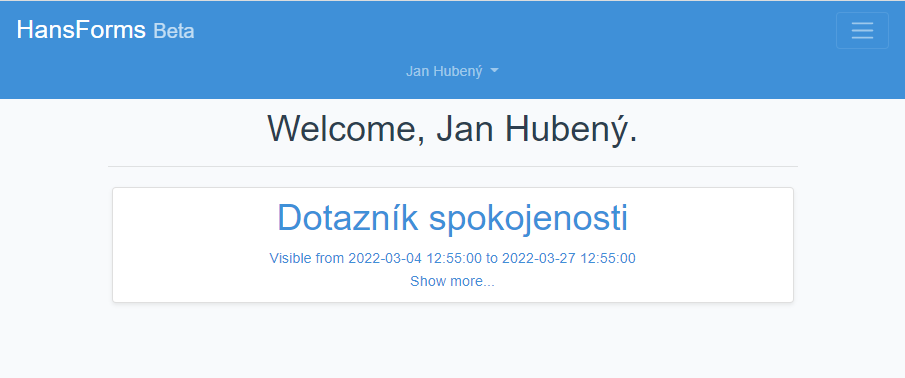
\includegraphics[width=0.95\textwidth]{img/pohledy/home.png}
			\caption{Pohled domovské stránky (přihlášený uživatel vlastnící formulář)}
			\label{fig:pohled_home}
		\end{figure}
	
		\subsubsection{Správa uživatele} %% Login, Register, Profile, ChangePassword, ResetPassword, ForgotPassword
		Co se týče administrativy nad uživatelem, existuje zde šest pohledů, které slouží k~různým účelům. Jedná se o~pohledy \textit{Login}, \textit{Register}, \textit{Profile}, \textit{ChangePassword}, \textit{ForgotPassword} a \textit{ResetPassword}.
		
		Pohled \textit{Login}, jak už z~názvu vyznívá, slouží k~přihlášení uživatele. Disponuje vstupními poli pro email a heslo. Poté, co uživatel klikne na tlačítko přihlášení, je na server poslán požadavek se získanými daty ze vstupních polí (na metodu \textit{login} viz sekce \ref{sec:user_login}). Pohled pak čeká na odpověď serveru - pokud obsahuje stavový kód 200, je přihlášený uživatel přesměrován na úvodní stránku aplikace. V~opačném případě je upozorněn na chybu, která se vyskytla (nejčastěji zpráva o~chybných údajích). Stránka také disponuje odkazem na stránku pro obnovu hesla. Díky metadatům na tento pohled nelze po přihlášení uživatele přistoupit.
		
		Oproti předchozímu pohledu pohled \textit{Register} slouží k~registraci uživatele. Obsahuje vstupní pole pro uživatelské jméno, email a heslo společně s~jeho ověřením. Po kliknutí na tlačítko pro registraci je poslán požadavek na server - konkrétně metodě \textit{register} (viz sekce \ref{sec:user_register}). Pokud je registrace úspěšná, je uživatel přesměrován na přihlašovací stránku. Pokud není, je mu vráceno oznámení s~chybou. Stejně jako v~pohledu \textit{Login} nelze po přihlášení uživatele na tento pohled přistoupit. 
		
		Dalším pohledem je \textit{Profile} (viz obrázek \ref{fig:pohled_profile}), který obsahuje náležité údaje o~přihlášeném uživateli (pokud uživatel není přihlášen, nelze k~němu přistoupit). Data o~uživateli získává ze serveru při načtení stránky pomocí metody \textit{show} (viz sekce \ref{sec:user_show}). Na tomto pohledu lze také změnit heslo (obsahuje tlačítko pro přesměrování na pohled pro změnu hesla) nebo celý účet smazat (při kliknutí na příslušné tlačítko po vyplnění hesla pro ověření se odešle požadavek na server na metodu \textit{destroy} viz sekce \ref{sec:user_destroy}).
		
		\begin{figure}[h]
			\centering
			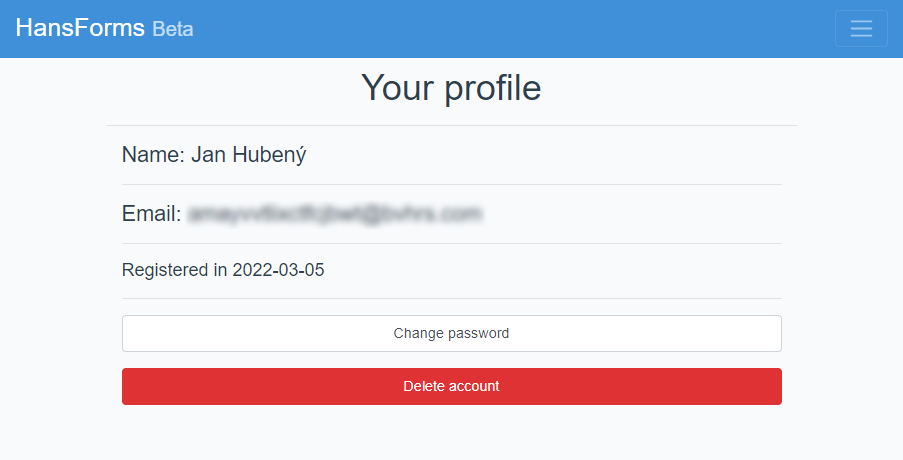
\includegraphics[width=0.95\textwidth]{img/pohledy/profile.png}
			\caption{Pohled profilu přihlášeného uživatele}
			\label{fig:pohled_profile}
		\end{figure}
		
		Již zmíněný pohled pro změnu hesla se jmenuje \textit{ChangePassword}. Na ten lze přistoupit pouze s~přihlášením. Obsahuje pole pro staré heslo, a pole pro heslo nové s~ověřením. Po kliknutí na příslušné tlačítko pro změnu hesla se odešle požadavek na server na metodu \textit{changePassword} viz sekce \ref{sec:user_changepassword}. Následně, na základě serverové odezvy, při úspěchu akce uživatele přesměruje na pohled \textit{Profile}. V~opačném případě je uživatel vyzván k~úpravě vyplněných údajů.
		
		Předposlední pohled v~této sekci je \textit{ForgotPassword}. Jedná se o~stánku, na kterou lze přistoupit z~pohledu \textit{Login}. Jak už z~názvu vyplývá, na tomto pohledu lze v~případě zapomenutého hesla požádat o~resetování - obsahuje vstupní pole pro vyplnění emailu, ke kterému je vázán účet se zapomenutým heslem, a tlačítko pro odeslání požadavku na server. Žádost o~obnovení se zasílá na metodu \textit{forgotPassword}, která je popsána v~sekci \ref{sec:user_reset_forgot_password}. Pokud vše proběhne bez problému, je uživatel přesměrován na domovskou stránku. Pokud se vyskytne chyba, je uživatel upozorněn.
		
		Posledním pohledem je \textit{ResetPassword}, který slouží k~resetování hesla tím, že se zvolí heslo nové. K~pohledu se přistupuje především prostřednictvím odkazu, který uživatel dostane na email (nelze k~pohledu přistoupit, když je uživatel přihlášen). V~pohledu je zobrazen email, ke kterému se vztahuje obnovení přístupu, kolonky pro vyplnění nového hesla s~potvrzením a příslušné tlačítko k~potvrzení úkonu - tedy k~odeslání požadavku na server. Po zpracování požadavku metodou \textit{resetPassword} (viz sekce \ref{sec:user_reset_forgot_password}) je vrácen příslušný stavový kód, na základě kterého je buď uživatel přesměrován (tj. v~případě úspěchu - kód 200) nebo upozorněn na chybu (tj. v~případě neúspěchu).
		
		\subsubsection{Formulář} %% Form
		Pohled \textit{Form} slouží k~zobrazení formuláře na základě jeho identifikátoru a zároveň nám umožňuje na zmíněný formulář odpovědět (viz obrázek \ref{fig:pohled_form}). Pohled je přizpůsoben na zobrazení jak veřejného formuláře, tak i privátního (to je rozlišeno na základě tvaru URL adresy). K~vykreslování všech otázek využívá komponentu \textit{FormElementsComponent} ze sekce \ref{sec:komp_form}.
		
		\begin{figure}[h]
			\centering
			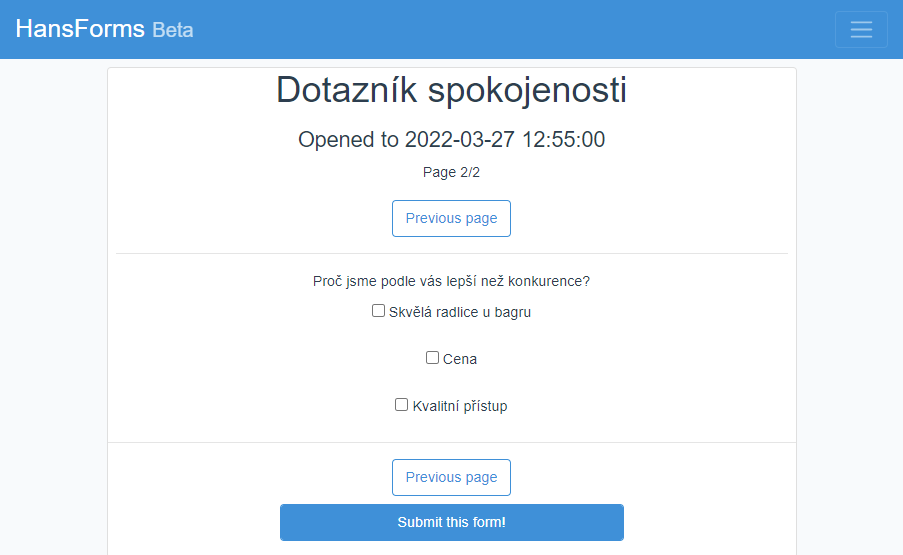
\includegraphics[width=0.95\textwidth]{img/pohledy/form.png}
			\caption{Pohled formuláře}
			\label{fig:pohled_form}
		\end{figure}
		
		Celý životní cyklus tohoto pohledu začíná tím, že pohled požádá server o~data formuláře na základě předaného identifikátoru (u~veřejného formuláře) nebo tokenu (u~privátního formuláře) v~URL adrese (u~veřejného formuláře pomocí metody \textit{show} ze sekce \ref{sec:form_show}, u~privátního pomocí metody \textit{privateShow} ze sekce \ref{sec:form_privateshow}). Pokud požadovaný formulář existuje, jsou příslušné otázky seřazeny a vykresleny (pokud ne, je oznámena chyba).
		
		Poté, co uživatel vyplní příslušná data a klikne na tlačítko pro uložení odpovědi, je odeslán další požadavek na server (pokud se jednalo o~veřejný formulář, tak směrující na metodu \textit{store} ze sekce \ref{sec:form_comp_public}, pokud se jednalo o~privátní formulář, tak pomocí metody \textit{privateStore} ze sekce \ref{sec:form_comp_private}). Na základě odpovědi serveru je respondent buď obeznámen s~úspěšným vyplněním formuláře a přesměrován na domovskou stránku, nebo je upozorněn na chybu a je vyzván k~opravě předávaných dat.
		
		\subsubsection{Tvorba formuláře}\label{sec:pohled_tvorba_formulare} %% CreateForm
		Pohled \textit{CreateForm} slouží k~vytvoření nového formuláře přihlášenému uživateli (nepřihlášený uživatel k~tomuto pohledu nemá přístup). 
		
		\begin{figure}[h]
			\centering
			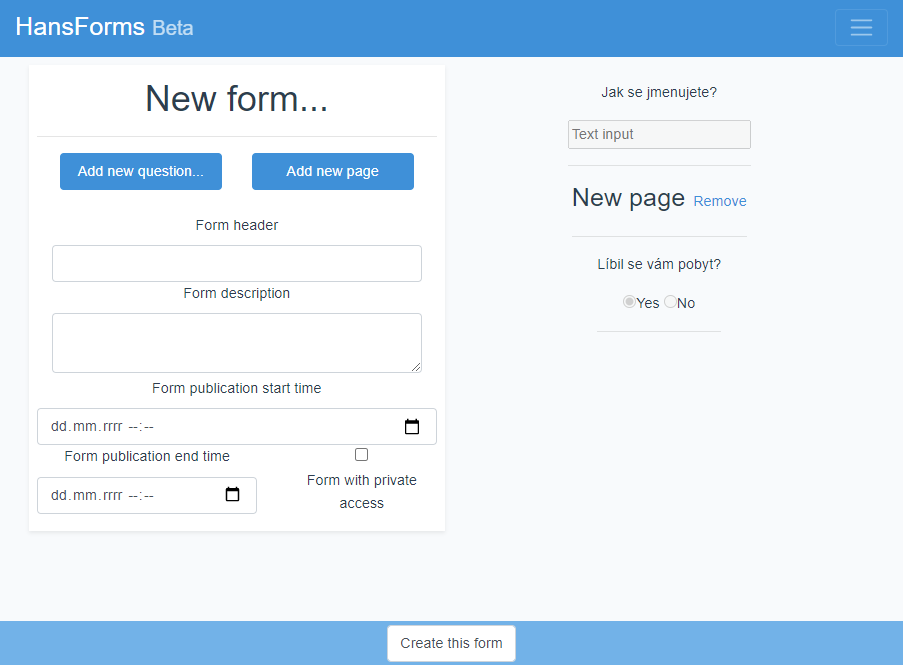
\includegraphics[width=0.95\textwidth]{img/pohledy/createform.png}
			\caption{Pohled pro vytvoření nového formuláře}
			\label{fig:pohled_createform}
		\end{figure}
		
		Z~grafické stránky je rozdělen na dvě části (viz obrázek \ref{fig:pohled_createform}) - první část obsahuje tlačítka pro přidání elementu otázky a elementu nové stránky a vstupní pole pro vyplnění základních údajů o~formuláři (tj. název a popisek formuláře, datum zveřejnění a datum ukončení zveřejnění, zda je formulář veřejný nebo privátní a u~privátního formuláře emaily, na které se zašle pozvánka), druhá část obsahuje grafický náhled na otázky. Ve spodní části je tlačítko určené k~ukončení úprav a odeslání dat vytvořeného formuláře na server (ta jsou zpracována metodou \textit{store} ze sekce \ref{sec:form_store}). Pokud tento požadavek projde bez problému, je uživatel přesměrován na domovskou stránku - v~opačném případě mu je předána příslušná chybová hláška.
		
		Pro úpravu otázek v~tomto návrhovém zobrazení je zřízeno modální okno \textit{ItemModal} (popsáno v~sekci \ref{sec:komp_modal}). To poté s~daty manipuluje pomocí dočasného úložiště \textit{createFormStore} a \textit{createFormChoicesStore} (ze sekce \ref{sec:data_prohlizec_form}). Data z~tohoto úložiště jsou průběžně předávána do pohledu, který je dynamicky vykresluje. Před odesláním jsou data validována a zpracována tak, aby splňovala podmínky zmíněné serverové metody, která je přijímá - na případné chyby je uživatel upozorněn.
		
		\subsubsection{Úprava formuláře}\label{sec:pohled_uprava_formulare} %% UpdateForm
		Pohled \textit{UpdateForm} slouží k~úpravě existujícího formuláře, který ještě nebyl publikován. K~tomuto pohledu má samozřejmě přístup jen vlastník existujícího formuláře.
		
		V~rámci vizuální i funkční stránky je skoro totožný s~pohledem \textit{CreateForm} - grafické rozložení stránky má stejné, používá stejná modální okna i dočasné úložiště. Jediné, v~čem se liší, je příjem dat existujícího formuláře, která jsou příslušně zpracována pro účely úprav formuláře, a způsob uložení úprav ve formuláři.
		
		Při inicializaci pohledu je nejprve vyhledán formulář, který má být upraven (pomocí serverové metody \textit{showWithAuth} ze sekce \ref{sec:form_showwithauth}). Pokud je nalezen, všechna jeho data jsou zpracována do stejného tvaru, který je používán i v~pohledu pro vytvoření formuláře (nutné kvůli využívání stejného dočasného úložiště a modálního okna). Poté, co je formulář uživatelem upraven dle jeho představ, je posílán požadavek se změněným formulářem na metodu \textit{update} (viz sekce \ref{sec:form_update}). Zpracování chyb je stejné jako ve zmíněném pohledu pro vytvoření formuláře.
		
		\subsubsection{Souhrn informací o~formuláři}\label{sec:pohled_souhrn_formulare} %% FormPreview
		Pohled \textit{FormPreview} slouží k~zobrazení souhrnu dat o~formuláři (viz obrázek \ref{fig:pohled_formpreview}). K~tomuto pohledu je přístup možný jen jako přihlášený uživatel (pro vykreslení příslušného souhrnu je samozřejmě nutné, aby požadovaný formulář přihlášenému uživateli patřil). Data o~formuláři jsou získána prostřednictvím metody \textit{showWithAuth} ze sekce  \ref{sec:form_showwithauth} - v~případě jakékoliv chyby je uživatel upozorněn konkrétním oznámením. V~rámci grafického rozložení je pohled rozdělen na dvě části. 
		
		V~první části jsou vypsány všechny základní údaje formuláře (tj. název a popisek, datum zveřejnění a datum ukončení zveřejnění, zda se jedná o~formulář veřejný nebo privátní - u~veřejného formuláře i odkaz k~vyplnění - a status zveřejnění - tzn. zda čeká na zveřejnění, zda je právě otevřený k~odpovědím či zda už zveřejnění bylo ukončeno). Také zde nalezneme ovládací prvky ve formě několika tlačítek, díky kterým můžeme formulář duplikovat (dále pomocí modálního okna \textit{FormDuplicationModal} ze sekce \ref{sec:komp_modal} a dočasného úložiště \textit{duplicateFormStore} ze sekce \ref{sec:data_prohlizec_form}), smazat (posláním požadavku na serverovou metodu \textit{destroy} ze sekce \ref{sec:form_destroy}), upravovat (možné jen v~případě, že formulář ještě nebyl zveřejněn - zajištěno přesměrováním na pohled \textit{UpdateForm} popsaný v~sekci \ref{sec:pohled_uprava_formulare}), měnit jeho přístupnost (dále pomocí modálního okna \textit{FormAccessibilityModal} ze sekce \ref{sec:komp_modal}) či prohlížet jeho výsledky (možné jen v~případě, že byl formulář už zveřejněn - zajištěno přesměrováním na pohled \textit{FormResults} ze sekce \ref{sec:pohled_vysledky_formulare}).
		
		Druhá část funguje jako interaktivní zobrazení formuláře (jsou zde vykresleny všechny otázky formuláře společně s~označením, kde začínají nové stránky) - lze zde např. testovat uživatelem definovaná validační pravidla pro vstupní data. Tato část je tvořena z~dat elementů formuláře, která jsou po přijetí předána komponentě \textit{FormElement} (viz sekce \ref{sec:komp_form}), která příslušné elementy vykreslí. Nelze pomocí této části přidávat data mezi odpovědi formuláře - data, která jsou v~tomto interaktivním zobrazení použita, se nikam neukládají.
		
		\begin{figure}[h]
			\centering
			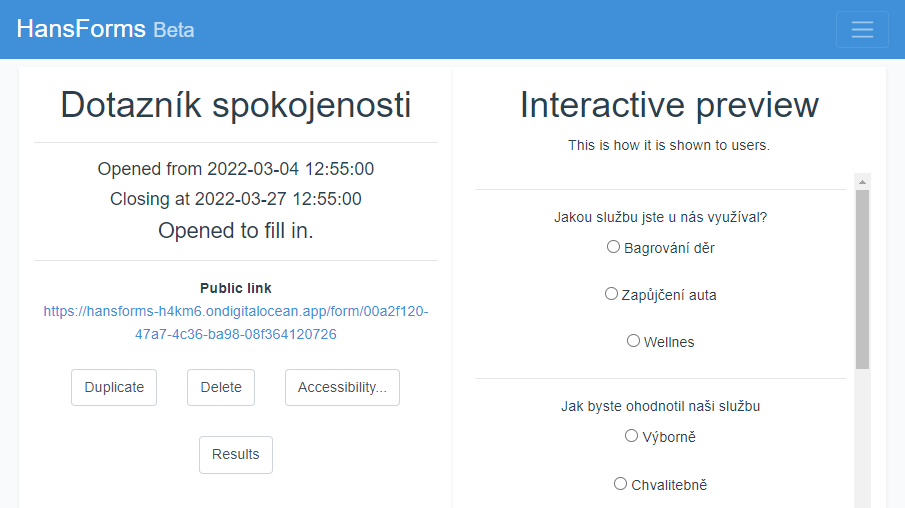
\includegraphics[width=0.95\textwidth]{img/pohledy/formpreview.png}
			\caption{Pohled souhrnu informací o~formuláři}
			\label{fig:pohled_formpreview}
		\end{figure}
		
		\subsubsection{Výsledky formuláře}\label{sec:pohled_vysledky_formulare} %% FormResults
		Pohled \textit{FormResults} slouží k~zobrazení všech odpovědí na formulář (tedy výsledků), a to i těch pro veřejnost (pokud je k~tomu formulář příslušně nastaven). Získání odpovědí pro vlastníka formuláře je zajištěno metodou \textit{index} ze sekce \ref{sec:form_comp_private_index}, pro veřejnost pomocí metody \textit{publicIndex}, která je popsána v~sekci \ref{sec:form_comp_public_index}. O~tom, jaká data mají být vrácena (zda má být vrácen výběr veřejných odpovědí nebo všechny odpovědi), rozhoduje tvar URL adresy. Pokud mají být vrácena všechna data, musí být vlastník samozřejmě přihlášen. V~případě chyby je uživatel příslušně obeznámen se stavem aplikace.
		
		Pokud byla data úspěšně přijata, můžeme na stránce vidět několik ovládacích prvků (tlačítko pro přesměrování na pohled domovské stránky nebo na pohled souhrnu informací o~formuláři, v~případě výsledků určených pro vlastníka formuláře tlačítko pro stažení vyexportovaných dat ve formátu MS Excel pomocí metody \textit{export} ze sekce \ref{sec:form_comp_export}, tlačítko pro změnu vykreslení výsledků - lze vybrat mezi komponentou \textit{ResultComponent} a \textit{DetailedResultsTable} ze sekce \ref{sec:komp_vysledky} - a tlačítko pro nastavení veřejných výsledků pomocí modálního okna \textit{FormResultsPublicationModal} ze sekce \ref{sec:modalni_okna_vysledky_form}) a samotné výsledky (viz obrázek \ref{fig:pohled_formresults}). Způsob vykreslení výsledků lze měnit mezi komplexní tabulkou se všemi odpovědmi \textit{DetailedResultsTable} a způsobem vykreslení výsledků \uv{co otázka, to všechny příslušné odpovědi} pomocí komponenty \textit{ResultComponent} (zde mohou být data zobrazena ve formě grafů - viz obrázek \ref{fig:pohled_formresults_graf} - nebo tabulky klíč/hodnota - záleží na typu).
		
		\begin{figure}[h]
			\centering
			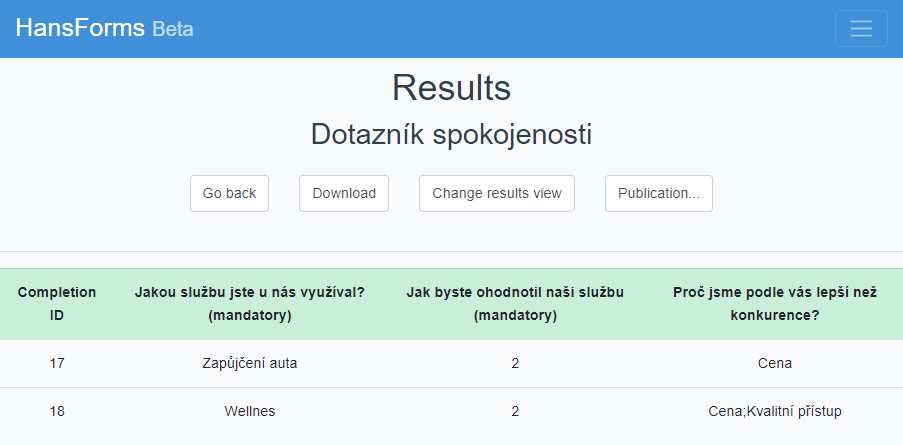
\includegraphics[width=0.95\textwidth]{img/pohledy/formresults.png}
			\caption{Pohled výsledků formuláře (pomocí komponenty \textit{DetailedResultsTable})}
			\label{fig:pohled_formresults}
		\end{figure}
	
		\begin{figure}[h]
			\centering
			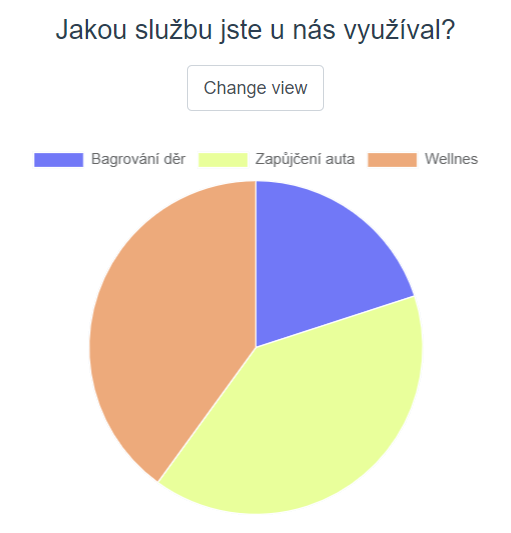
\includegraphics[width=0.5\textwidth]{img/pohledy/formresults_graf.png}
			\caption{Komponenta \textit{ResultComponent} vykreslující koláčový graf}
			\label{fig:pohled_formresults_graf}
		\end{figure}
		
		\subsubsection{Ostatní pohledy} %% NotFound, About
		Poslední pohledy, které v~aplikaci existují, jsou \textit{NotFound} a \textit{About}. Jedná se o~statické pohledy - obsahují jen předepsaný obsah tedy nedisponují nějakou specifickou funkcionalitou. 
		
		Pohled \textit{About} je použit pro stručný popis projektu. Pohled \textit{NotFound} je určen k~vykreslení v~případě, že směrovač (viz sekce \ref{sec:fe_router}) požadovanou cestu nezná. Obsahuje jen text indikující, že požadovaná stránka nebyla nalezena.
